%% DONE
\id{МРНТИ 28.23.17}{https://doi.org/10.58805/kazutb.v.1.26-599}

\begin{articleheader}
\sectionwithauthors{Н.О.Мекебаев,  Д.К.Даркенбаев, Н.А. Модовов , Ж.А. Орынтаева}{КЛАССИФИКАЦИЯЛЫҚ АЛГОРИТМДЕРДІ ҚОЛДАНЫП ДАУЫСТЫ ТАНУ}

{\bfseries
\textsuperscript{1}Н.О. Мекебаев\textsuperscript{\envelope } \alink{https://orcid.org/0000-0002-9117-4369},
\textsuperscript{2}Д.К. Даркенбаев\alink{https://orcid.org/0000-0002-6491-8043},
\textsuperscript{1}Н.А. Модовов\alink{https://orcid.org/0009-0005-1642-9834},
\textsuperscript{1}Ж.А. Орынтаева\alink{https://orcid.org/0000-0002-1993-9566}}
\end{articleheader}

\begin{affiliation}
{\em \textsuperscript{1}Қазақ ұлттық қыздар педагогикалық университеті, Алматы, Қазақстан,}

{\em \textsuperscript{2}Әл-Фараби атындағы Қазақ ұлттық университеті, Алматы, Қазақстан}

\raggedright \textsuperscript{\envelope }{\em Корреспондент-автор: \href{mailto:nurbapa@gmail.com}{\nolinkurl{nurbapa@gmail.com}}}
\end{affiliation}

Дауыс тану жүйелері машиналық оқыту әдістеріне негізделген, оның ішінде
классификациялық алгоритмдер кеңінен қолданылады. Классификация дауыс
сигналдарын әртүрлі санаттарға, мысалы, сөздер немесе сөйлемдерге бөліп
тануды жүзеге асырады. Бұл үдерісте жиі қолданылатын алгоритмдерге
логистикалық регрессия, шешім ағаштары және нейрондық желілер жатады.
Дауыс сигналын өңдеуде алдымен ерекшеліктері, яғни маңызды параметрлері,
экстракцияланады, содан кейін олар классификаторға беріледі.
Классификация нәтижесінде жүйе сөйлеген сөзді мәтінге түрлендіреді
немесе дыбыстың нақты мазмұнын анықтайды. Бұл технология адам-компьютер
өзара әрекеттестігін жақсарту үшін маңызды. Бұл мақалада машиналық оқыту
әдістерін қолдана отырып, сөйлеушінің даусын анықтау мәселесін шешу үшін
жіктеу алгоритмдерін қарастырамыз. Сөйлеудің алдын ала өңдеуде МҒСС-ті
алгортимін пайдаландық. Жоғарыдағы мәселені шешу үшін бес жіктеу
алгортмі қарастырылып, салыстырмалы талдау жасалды. Алғашқы эксперимент
жасағанда ең жақсы нәтиже көрсеткен SVC алгортимі 0,90 және MLP
Classifier алгоритмі 0,83 нәтижелерін көрсетті. Келесі экспермиентте
жеке тұлғаның дауысын анықтауда неғұрлым үлкен дәлдікте Robust scaler
әдісімен масштабтауда -- 0,93 көпқабатты персептрон көрсете бастады.
Сондықтан бұл мәселені шешу үшін сөйлеу сигналының ерекшелігін ескеретін
көп қабатты перцептронды қолдануға болады.

{\bfseries Түйін сөздер:} алгоритм, дауыс, сөйлеуді тану, ASR, MFCC, MLP.

\begin{articleheader}
{\bfseries РАСПОЗНАВАНИЕ ГОЛОСА С ПОМОЩЬЮ АЛГОРИТМОВ КЛАССИФИКАЦИИ}

{\bfseries
\textsuperscript{1}Н.О. Мекебаев\textsuperscript{\envelope },
\textsuperscript{2}Д.К. Даркенбаев,
\textsuperscript{1}Н.А Модовов,
\textsuperscript{1}Ж.А. Орынтаева}
\end{articleheader}

\begin{affiliation}
{\em \textsuperscript{1}Казахский национальный женский педагогический университет, Алматы, Казахстан,}

{\em \textsuperscript{2}Казахский национальный университет им. Аль-Фараби, Алматы, Казахстан,}

{\em e-mail: \href{mailto:nurbapa@gmail.com}{\nolinkurl{nurbapa@gmail.com}}}
\end{affiliation}

Системы распознавания речи основаны на методах машинного обучения, среди
которых широко применяются классификационные алгоритмы. Классификация
выполняет задачу разделения голосовых сигналов на различные категории,
такие как слова или предложения. К часто используемым алгоритмам
относятся логистическая регрессия, деревья решений и нейронные сети. В
процессе обработки голосового сигнала сначала извлекаются его
особенности, то есть важные параметры, которые затем передаются
классификатору. По результатам классификации система преобразует речь в
текст или определяет конкретное содержание звука. Эта технология важна
для улучшения взаимодействия человека с компьютером. В данной статье
обсуждается алгоритм классификации для задачи идентификации речи с
использованием метода машинного обучения. Алгоритм MFCC используется для
предварительной обработки речи. Для решения этой задачи проведен
сравнительный анализ пяти алгоритмов классификации. В первом
эксперименте были определены методы опорного вектора -- 0,90 и
многослойного перцептрона -- 0,83 и показаны лучшие результаты. Во
втором эксперименте был предложен многослойный перцептрон с точностью
0,93 с использованием метода Робастного скалера для идентификации
личности. Поэтому для решения этой проблемы можно использовать
многослойный персептрон, учитывающий детали аудиосигнала.

{\bfseries Ключевые слова:} алгоритм, голос, распознавание речи, ASR, MFCC,
MLP.

\begin{articleheader}
{\bfseries VOICE RECOGNITION USING CLASSIFICATION ALGORITHMS}

{\bfseries
\textsuperscript{1}N. Mekebayev\textsuperscript{\envelope },
\textsuperscript{2}D. Darkenbayev,
\textsuperscript{1}N. Modovov,
\textsuperscript{1}Zh. Oryntaeva}
\end{articleheader}

\begin{affiliation}
{\em \textsuperscript{1}Kazakh National Women' s Pedagogical University, Almaty, Kazakhstan,}

{\em \textsuperscript{2}Al-Farabi Kazakh National University, Almaty, Kazakhstan,}

{\em e-mail: \href{mailto:nurbapa@gmail.com}{\nolinkurl{nurbapa@gmail.com}}}
\end{affiliation}

In Speech recognition systems are based on machine learning methods,
among which classification algorithms are widely used. Classification
performs the task of dividing voice signals into various categories,
such as words or sentences. Commonly used algorithms include logistic
regression, decision trees, and neural networks. During voice signal
processing, features, i.e., important parameters, are first extracted
and then passed to the classifier. Based on the classification results,
the system converts speech into text or determines the specific content
of the sound. This technology is essential for improving human-computer
interaction.This article discusses a classification algorithm for the
problem of speech identification using the machine learning method. The
MFCC algorithm is used for preprocessing speech. To solve this problem,
a comparative analysis of five classification algorithms was carried
out. In the first experiment, the methods of the reference vector --
0.90 and the multilayer perceptron -- 0.83 were determined and the best
results were shown. In the second experiment, a multilayer perceptron
with an accuracy of 0.93 was proposed using the Robust Scaler method for
personality identification. Therefore, a multilayer perceptron can be
used to solve this problem, taking into account the details of the audio
signal. be used, taking into account the details of the audio. signal.

{\bfseries Keywords:} algorithm, voice, speech recognition, ASR, MFCC, MLP.

\begin{multicols}{2}
{\bfseries Кіріспе.} Ауыз екі сөйлеу тілін тану -- аудиодағы сөйлеуші
сөйлейтін тілді жіктеу мәселесі. Ол әдетте сөздің тілдік санатын
бастапқыда анықтау үшін, кейіннен өңдеуді жеңілдету үшін көптілді
автоматты сөйлеуді тану (ASR) сияқты көптілді сөйлеуді өңдеу
тапсырмаларының алдыңғы бөлігі ретінде пайдаланылады. Тұрақты және
сенімді тілді сәйкестендіру жүйесі бұл жүйелерде жоғары өнімділік пен
дәлдікке жетудің кілті болып табылады {[}1{]}.

Зерттеудің мақсаты сөйлеушінің дауысын анықтауға арналған машиналық
оқытудың классификациялық әдістерін зерттеу. Осы мақсатқа жету үшін
келесі міндеттер орындалды. Классификация алгоритміне салыстырмалы
талдау жүргізіліп бірқатар жіктеу алгоритмдері және сөйлеуді алдын ала
өңдеу мәселелері қарастырылды {[}2{]}.

Дәстүрлі тілдік анықтау көбінесе акустикалық және фонетикалық
ерекшеліктерге сүйенеді. Жалпы акустикалық сипаттамаларға, басқалармен
қатар, кепстральды мель-жиілік коэффициенттері (MFCC), дельта
коэффициенттері, перцептивті сызықтық болжау коэффициенттері (PLP) және
кепстральды гамма-жиілік коэффициенттері жатады {[}3{]} .

Соңғы жылдары cөйлеуді автоматты түрде тану (ASR), визуалды сөйлеуді
тану ((VST) және аудиовизуалды сөйлеуді тану (AVSR) салаларында ауқымды
ғылыми-зерттеу жұмыстары жүргізілуде {[}4{]}.

Бұл мақалада дауысты (сөйлеу екі тілді) тануды қарастырамыз. Тілді тану
-- бұл сөйлеушіні тануға ұқсас мәселе, өйткені біз белгілі бір сөздің
мазмұны туралы емес, бүкіл мәлімдеме туралы ақпарат алуға тырысамыз.
Жіктеу алгортимдері техникасындағы дауысты (тілді) тануға қолдану біздің
әдістеріміздің жан-жақты екенін және сөйлеудің бірнеше саласында
әлеуетті қолданылатынын көрсетеді {[}5{]}.

Қазақстанда қазақ тілінің сөйлеу технологиялары зерттелуде. Қазақ тілі
агглютинативті тілдер тобына жатады. Агглютинативті тілдердің
құрылымында әр түрлі форматтағы қосымшалар (жұрнақтар, жалғаулар)
бірінен соң бірі кезектесіп қосылады, бұл сөзді өзгертудің басым түрі
болып табылады және осы қосымшалардың әрқайсысы тек бір мағынамен
жүктеледі {[}6{]}. Түрік, моңғол, корей тілдері агглютинативті тілдерге
жатады. Біздің елімізде қазақ тіліндегі тұлғаны тану жүйесі әлі
дамымаған, бұл аталған бағыттағы зерттеулерді өзекті етеді.

Бұл мақалада жіктеу алгоритмдерін қолдана отырып, дауысты тану, анықтау
міндеттерін қарастырамыз.

{\bfseries Материалдар мен әдістер.} Сөйлеуді тану үдерісі негізінде
алдын ала өңдеуден тұрады {[}7{]}. Осы мақалада біз дауыстың динамикалық
өңдеуде МҒСС-ті қолданамыз. Сөйлеу сигналының алдын-ала өңдеу үдерісі
1-ші суретте көрсетілген. MFCC (Mel-Frequency Cepstral Coefficients) мел
жиілігінің кепстральды коэффициенттері дауыс, дыбыспен жұмыс жасау
кезінде ең танымал таңдау болып табылады. Бұл тәсілдің ерекшелігі -
бастапқы сигналдың ұзындығынан алынған сипаттамалар векторы және ондағы
сөйлейтін жеке ерекшеліктердің таралуын есепке алу {[}8{]}.
\end{multicols}

\begin{figure}[H]
	\centering
	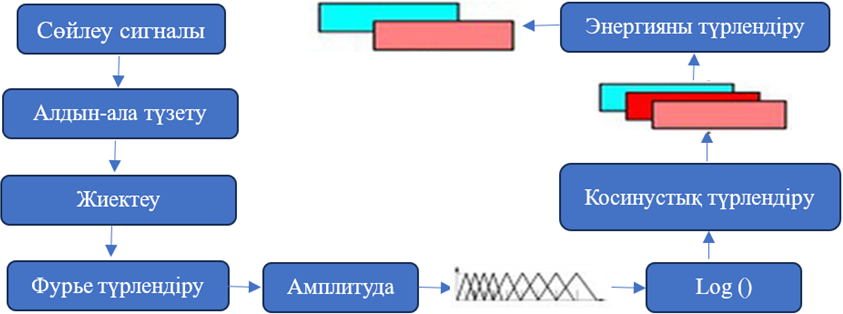
\includegraphics[width=0.8\textwidth]{media/ict/image5}
	\caption*{1 - сурет. Сөйлеу сигналын алдын ала өңдеу}
\end{figure}

\begin{multicols}{2}
Әрбір жазылған аудио негізінде 5806 белгі алынды. Аудио файлдағы әрбір
кез-келген дауыс жазылып жатқан сигнал динамиктің белгі атымен
белгіленеді. Осы алынған дерек, мәліметтер жиынының жалпы өлшемі
1285x5806.

Кепстр - бұл сүзгіні дыбыс толқынының көзінен бөлетін түрлендіру.

Көрсетілгенді визуализациялау үшін 5806 белгісі бар векторлық
кеңістіктің және екі-үш өлшемді кеңістіктің өлшемдерін азайту үшін
негізгі компоненттер әдісі қолданылады. Дисперсияны негізгі компонент
әдісімен кішірейтілген мөлшерде сақтау 2-суретте көрсетілген.
\end{multicols}

\begin{figure}[H]
	\centering
	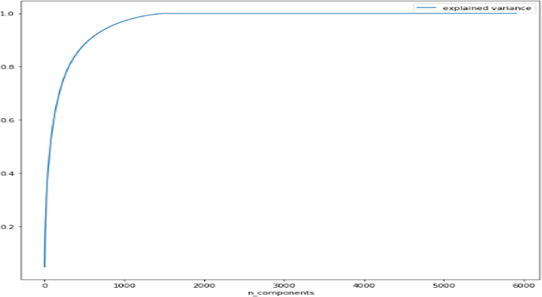
\includegraphics[width=0.8\textwidth]{media/ict/image6}
	\caption*{2 - сурет. Негізгі құрамдас әдісті пайдаланып өлшемділікті азайту кезінде дисперсияны сақтау}
\end{figure}

\begin{multicols}{2}
Жоғарыда келтірілген графикте көрсетілгендей, деректердің өлшемі 1285
белгіге дейін төмендеген жағдайда дисперсия 98,9 \% сақталады. Алайда,
жіктеу модельдерімен және деректер стандарттаушыларымен жүргізілген
тәжірибе көрсеткендей, бұл кішірейту конструктивті түрде жіктеудің
дәлдігіне ықпал етеді.

{\bfseries Материалдар мен әдістер.} Эксперимент жасау үшін деректерді
«Ақпараттық және есептеуіш технологиялар» инситутының зерттеушілерінің
базасынан алынды {[}9{]}. Берілген деректер, мәліметтер жиынтығы 0-19
сөйлеушінің 1285 аудио жазбасынан тұрды, олардың әрқайсысы 68-76
сөйлемнен тұратын жазбаны жазды. Қазақ тіліндегі әрбір аудиожазба орта
есеппен 5 секундқа созылатын сөз тіркесін білдіреді. Сөйлеушіні тану
үшін біз келесі деректер, мәліметтерді жинадық: сөйлеушінің аты,
сөйлеушінің жынысы, сөйлеушінің туған жері, сөйлеушінің туған жылы.
Төмендегі 1 кестеде сөйлеушінің мәліметтері көрсетілген.
\end{multicols}

\begin{table}[H]
\caption*{1 - кесте. Сөйлеушінің мәліметтері}
\centering
\begin{tblr}{
  cell{2}{2} = {c},
  cell{2}{3} = {c},
  cell{2}{4} = {c},
  cell{2}{5} = {c},
  cell{2}{6} = {c},
  cell{2}{7} = {c},
  cell{3}{2} = {c},
  cell{3}{3} = {c},
  cell{3}{4} = {c},
  cell{3}{5} = {c},
  cell{3}{6} = {c},
  cell{3}{7} = {c},
  cell{4}{2} = {c},
  cell{4}{3} = {c},
  cell{4}{4} = {c},
  cell{4}{5} = {c},
  cell{4}{6} = {c},
  cell{4}{7} = {c},
  cell{5}{2} = {c},
  cell{5}{3} = {c},
  cell{5}{4} = {c},
  cell{5}{5} = {c},
  cell{5}{6} = {c},
  cell{5}{7} = {c},
  cell{6}{2} = {c},
  cell{6}{3} = {c},
  cell{6}{4} = {c},
  cell{6}{5} = {c},
  cell{6}{6} = {c},
  cell{6}{7} = {c},
  hlines,
  vlines,
}
ТАӘ & Тегі & Аты & Әкесінің аты & Жынысы & Туған жері & Туған жылы\\
МЖА & Масимканова & Жазира & Ауезбеккызы & әйел & Алматы & 20.03.1982\\
ИМТ & Искакова & Молдир & Тасболаткызы & әйел & Алматы & 01.01.1994\\
ДАЖ & Дүйсенбаева & Айгерім & Жанболаткызы & әйел & Алматы & 15.05.1995\\
ЖЕА & Жетписбаев & Ерлан & Алибекович & ер & Алматы & 23.05.1995\\
ССМ & Самрат & Санжар & Мұхаметқалиулы & ер & Алматы & 12.07.1996
\end{tblr}
\end{table}

\begin{multicols}{2}
\emph{Жіктеу алгоритмдері}

Сөйлеушіні анықтау тану мәселесін шешуде төмендегідей жіктеу
алгоритмдерін қарастырдық:

\emph{MLP Classifier алгоритмі}

MLP көп қабатты перцептрон -
\((Y) = T_{n}:{\ \ T}_{n} \rightarrow T^{0}\) функциясын аудио деректер
сериясында оқыту арқылы зерттейтін басқарылатын оқыту алгоритмі, мұндағы
n - енгізу үшін өлшемдер саны, а\textsubscript{0}-шығару үшін өлшемдер
саны. \(Y = y_{1},y_{2},\ldots,y_{n}\) функцияларының жиынтығын ескере
отырып ` \(y_{n}\)' ол кез-келген классификация үшін сызықтық емес
функциялардың жуықтауын зерттей алады. 3-ші суретте MLP архитектурасы
көрсетілген.
\end{multicols}

\begin{figure}[H]
	\centering
	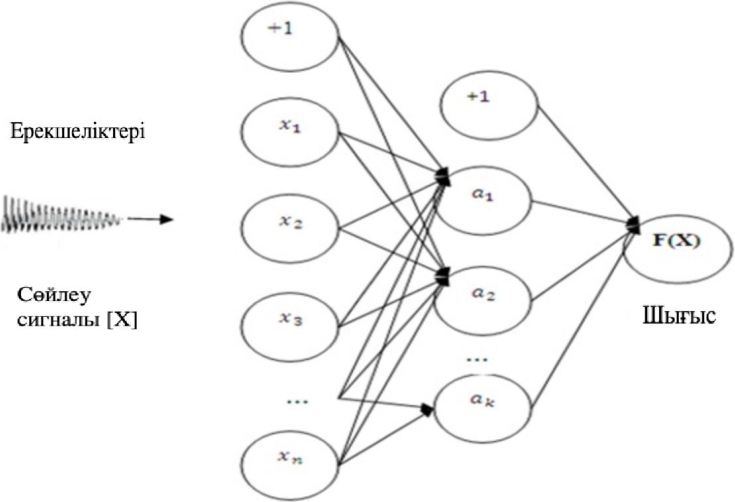
\includegraphics[width=0.55\textwidth]{media/ict/image7}
	\caption*{3 – сурет. MLP архитектурасы}
\end{figure}

\begin{multicols}{2}
Кіріс қабаты кіріс функцияларын білдіретін
\(x_{1},\ x_{2},\ ...,x_{n\ }\ \)тұрады. Шығыс қабаты соңғы жасырын
қабаттан мәндерді алады және оларды шығару мәндеріне түрлендіреді.

\emph{Extra-Trees алгортимі}

Extra-Trees алгоритмі жаңартылмайтын шешімдер немесе регрессиялар
ансамблін жасайды. Қадамға негізделген ансамбльдің басқа әдістері
алгоритмнің екі негізгі айырмашылығы-ол кездейсоқ түрде кесу нүктелерін
таңдап, түйіндерді сындырады және қадамдарды ұлғайту үшін бүкіл оқу
үлгісін пайдаланады {[}10{]}.

\emph{Trees\_node(M)}

Тұрақты оқыту жиынтығы N түйініне сәйкес келіп кіріс синалын айналады.

шығыс синалы ретінде {[}\(d\) \textless{} \(d_{c}\){]} аламыз

-- оқытуда \emph{Tree(S.)} ақиқат болған жаңдайда ешнәрсе қайтарылмайды

-- ондай жағдайда тұрақты емес барлық (S) атрибуттарының топтарының
ішіндегі \{\(d_{1}\),...\({,d}_{K}\)\} атрибуттарын тұрақты түрде
таңдаймыз;

-- осы K қадамдарды \{g\textsubscript{1},...,g\textsubscript{K} \}
таңдап, мұндағы g\textsubscript{i} = \emph{Random\_split.}(G,
d\textsubscript{i}), ∀ i = 1,..., K.;

-- g\textsubscript{∗} сегменттерінде Score(g\textsubscript{∗}, G.) =
max\textsubscript{i=1,...,K} Score(g\textsubscript{i}, G.) деп
келтіреміз.

\emph{Random\_split.(S,} \(a\)\emph{)}

G ішкі жиыны және d атрибуты кірісі.

-- \(d_{\max}^{G}\) және \(d_{\min}^{G}\) минималды мәнді, максималды
мәнін G-ге біріктіреді;

\emph{Tree(S.)}

G ішкі жиынның кірісі

\(d\) логикалық мәні шығысы

-- егерде \textbar{} G \textbar{} \textless{} n\textsubscript{min} болса
қайтару ақиқатты көрсетеді;

-- егер барлық G атрибуттары тұрақты болса, біз TRUE (ақиқат)мәнін
қайтарамыз;

-- егер G шығысы тұрақты болса, біз true (ақиқат)қайтарамыз;

-- болмаған жағдайда біз false (жалған) мәнін қайтарамыз.

Оның екі параметрі бар: K әр түйін үшін кездейсоқ таңдалған атрибуттар
саны және n\textsubscript{min} түйінді бөлу үшін ең кіші үлгінің өлшемі.
Ол ансамбль моделін құру үшін бастапқы оқыту моделімен бірнеше рет
қолданылады {[}11{]}.

\emph{SVC алгоритмі}

Сызықтық бөлінетін екілік жіктеу мәселесін шешу үшін SVC пайдалану үшін
бізге қажет:

-- \emph{J}-ді құруда, мұндағы
\(J_{ij} = z_{i}z_{j}y_{i} \cdot y_{j}\)

-- σ --ны табу;

-- \(\sum_{i = 1}^{M}{}{\sigma}_{i} - \frac{1}{2}{\sigma\ }^{T}J\sigma\ \)

-- \({\sigma\ }_{i} \geq 0 \forall_{i} \text{ және }\sum_{i = 1}^{M}{}{\sigma}_{i}z_{i} = 0\) осы
шектеу аймақтарын ескере қарап, мейілінше жоғарылату;

-- QN шешімді қолдану болып табылады;

-- \(v = \sum_{i = 1}^{M}{}{\sigma}_{i}z_{i}y_{i}\) есептеу;

-- \({\sigma}_{i} > 0\) индекстерін есептеп, \emph{l} тірек
әрбір векторының санын анықтау;

-- \(a = \frac{1}{M_{s}}\sum_{l \in L}^{}{}({\sigma\ }_{m}z_{m}y_{m} \cdot y_{L}\)
есептеу керек;

-- \(y^{'}\ \)кез-келген нүктесі \(z^{'} = sgn(v \cdot y^{'} + a\)
есептеу тәсілімен жіктеуге болады.

\emph{Gaussian NB алгоритмі}

Осы Naive Bayes - \(y_{1}, y_{2}, \ldots, y_{n}\) тізбегіндегі
көбейтіндісіне с пропорционал \(А_{k}\)класының ішінде жататын
\(m + 1\) деректер нүктесінің нақты ықтималдығын береді. \(m\)
алдыңғы \(\sigma\left( A_{k} \right) -\) класы мен
\(\sigma\left( А_{a} \right)\prod_{i = 1}^{m}{}\sigma\left( A_{k} \right)\ \)белгілерінің
арасындағы шартты ықтималдығы болып табылады {[}12{]}.

\[\sigma(A_{a})\prod_{i = 1}^{m}{}\sigma\left( A_{a} \right) > \sigma(A_{b})\prod_{i = 1}^{m}{}\sigma(y_{i}\vee A_{b})\]

\[\sigma\left( y_{1},\ldots,y_{n} \right) > \sigma(A_{b}\vee y_{1},\ldots,\ y_{n})\]

Осылайша, \(y_{1},\ y_{2},\ ...,y_{n\ }\ \) мәліметтер нүктесіне кластың
осы ең ықтимал нақты тағайындалуы \(a = 1,\ldots,A\) үшін
\(\sigma\left( A_{a} \right)\prod_{i = 1}^{m}{}\ \sigma\left( A_{k} \right)\ \)есептеудің
мәні макисмум болып табылатын \(A_{k}\ \)класындағы
\(y_{1},\ y_{2},\ ...,y_{n\ }\ \)есептеу ықтималдығы.

\emph{KNN алгоритмі}

KNN алгоритмі сұрау көрінісі мен мәліметтер жиынтығындағы көрініс
жиынтығы арасындағы ара қашықтықты өлшейді.

Тестілеу модельдеу нысандарының әрқайсысын жіктеу үшін келесі
әрекеттерді жүйелі түрде орындау қажет:

- оқыту моделінің әрбір нысанына дейінгі ара қашықтықты есептеу керек;

- K-ны оқыту моделінің нысанын таңдау керек;

- К классификацияланған объектінің класы жақын көршілер арасында ең көп
таралған класс болып табылады.

Жоғарыдағы ұсынылған алгоритмдер тұлғаны сәйкестендіру, сөйлеушіні тану
мәселесіне қолданылып, салыстырмалы талдау жүргізілді. Салыстырмалы.
талдаулар мен эксперименттер олардың ең жақсы екенін көрсетеді.
Нәтижелерінде тірек векторлық машиналар мен көп қабатты перцептронды
қолдану арқылы алынды. 4-ші суретте осы мәліметтер жиынының жіктеу
дәлдігі көрсетілген.
\end{multicols}

\begin{figure}[H]
	\centering
	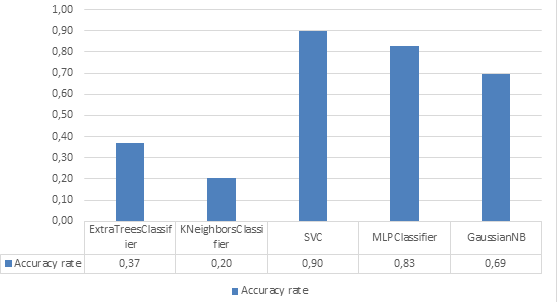
\includegraphics[width=0.7\textwidth]{media/ict/image8}
	\caption*{4 -- сурет. Деректер жиынының жітеу дәлдігі}
\end{figure}

\begin{multicols}{2}
4-ші суреттен көрініп тұрғандай тірек векторлық машина мен көпқабатты
перцептрон ең жақсы нәтиже көрсетті -- сәйкесінше 0,90 және 0,83.

Нәтижелерді жақсарту үшін біз әртүрлі әдістерді қолданып масштабтау
жасап, нәтижелердің өзгергені байқалды. 5 -- суретте әртүрлі әдістерді
қолдану арқылы деректерді масштабтау кезіндегі жіктеу дәлдігі
көрсетілген.
\end{multicols}

\begin{figure}[H]
	\centering
	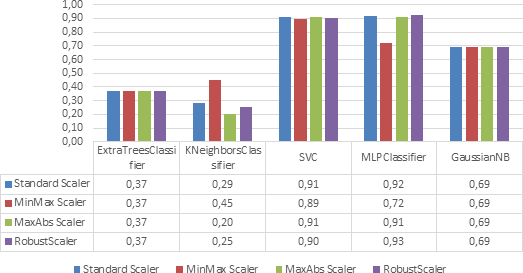
\includegraphics[width=0.7\textwidth]{media/ict/image9}
	\caption*{5 - сурет. Әртүрлі әдістерді қолдану арқылы деректерді масштабтау кезіндегі жіктеу дәлдігі}
\end{figure}

\begin{multicols}{2}
Көпқабатты перцептрон сенімді Robust scaler әдісін қолданып масштабтаған
кезде ең жоғары дәлдікке 0,93 жетті, ал тірек векторлық машиналар
дәлдігі азая бастады, бірақ Standard scaler және MaxAb Scaler әдісімен
масштабтау кезінде дәлдік нәтижелері 0,90-нан 0,91-ге дейін жақсарды.

Сөйлеу нысандарының өлшемділігін 1390-ға дейін азайту үшін негізгі
құрамдас талдауды пайдалансаңыз, жіктеу дәлдігі 2-кестеде көрсетілгендей
өзгереді.
\end{multicols}

\begin{figure}[H]
	\centering
	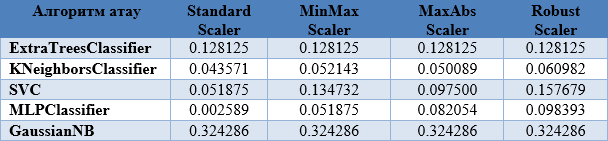
\includegraphics[width=0.9\textwidth]{media/ict/image10}
	\caption*{2 - кесте. Өлшемді азайту арқылы деректер бойынша жіктеу дәлдігі}
\end{figure}

\begin{multicols}{2}
Салыстырмалы талдаудың мақсаты жеке сөйлеушіні тану мәселесіне жіктеу
алгоритмінің әсер ету дәрежесін анықтау, сонымен қатар SVC және MLP
жіктеуіш алгоритмдерін салыстырмалы бағалау болды. Дауыс деректерінің
үлгілерін оқыту бойынша жүргізілген эксперименттер осы алгоритмдердің
келешегі туралы айтуға мүмкіндік беретін нәтижелерді көрсетеді. Алынған
мәліметтер 6 және 7-суреттерде берілген.
\end{multicols}

\begin{figure}[H]
	\centering
	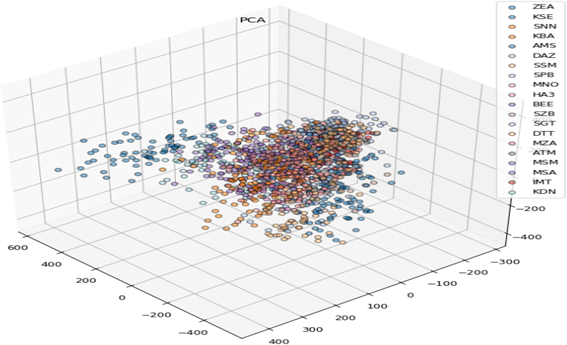
\includegraphics[width=0.9\textwidth]{media/ict/image11}
	\caption*{6 - сурет. Дыбыстық деректердің, сөйлеу белгілерінің үш өлшемді көрінісі}
\end{figure}

\begin{figure}[H]
	\centering
	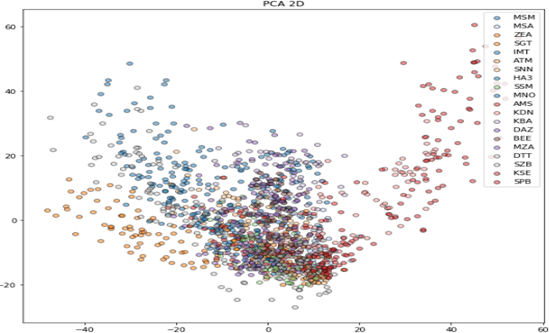
\includegraphics[width=0.9\textwidth]{media/ict/image12}
	\caption*{7 - сурет. Дыбыстық деректердің, сөйлеу белгілерінің екі өлшемді көрінісі}
\end{figure}

\begin{multicols}{2}
Әртүрлі әдістерді қолдану арқылы деректерді, масштабтау кезіндегі жіктеу
нәтижелері алдын ала экспериментте алынған нәтижелерден айтарлықтай
ерекшеленетіні анықталды.

{\bfseries Қортынды.} Бұл мақалада біз бірнеше жіктеу алгоритмдерін және
сөйлеуді алдын ала өңдеу мәселесін қарастырдық. Тәжірибе нәтижелерін
талдау негізінде Robust scaler әдісімен масштабтау үшін дәлдігі 0,93
көпқабатты перцептрон ұсынылады, ал сөйлеу сигналын көпқабатты
перцептрон көмегімен жіктеуге болатындығы анықталды. Содан кейін алынған
деректерге сүйене отырып, сөйлеушіні тану үдерісін анықтадық.

Әрі қарайғы зерттеу барысында біз алынған мәліметтердің шынайылығын
тексеру мәселесін шешеміз деп үміттенеміз.
\end{multicols}

\begin{center}
{\bfseries Әдебиеттер}
\end{center}

\begin{references}
1. Matejka, P.; Zhang, L.; Ng, T.; Glembek, O.; Ma, J.; Zhang, B.;
Mallidi, S.H. Neural Network Bottleneck Features for Language
Identification // In Proceedings of the Speaker and Language
Recognition Workshop (Odyssey 2014). - Joensuu, Finland, 16--19 June
2014. -P. 299--304. DOI: 10.21437/Odyssey.2014-45

2. Pliakos K., Geurts P., Vens C. Global multi-output decision trees for
interaction prediction // Machine Learning. - 2018.- P. 1--25.
DOI:10.1007/s10994-018-5700-x

3. \href{https://www.scopus.com/authid/detail.uri?authorId=55967630400}{Mamyrbayev,
O.},~\href{https://www.scopus.com/authid/detail.uri?authorId=57200275502}{Toleu,
A.},~\href{https://www.scopus.com/authid/detail.uri?authorId=57200276217}{Tolegen,
G.},~\href{https://www.scopus.com/authid/detail.uri?authorId=57202316868}{Mekebayev,
N.}, Neural architectures for gender detection and speaker
identification//Cogent Engineering.- 2020.-Vol.7(1).

\href{https://doi.org/10.1080/23311916.2020.1727168}{DOI
10.1080/23311916.2020.1727168}

4. R. Wolff, " MonkeyLearn Blog," 5 Types of Classification Algorithms
inMachine Learning, 26 August 2020.

5. \href{https://www.scopus.com/authid/detail.uri?authorId=56153126500}{Kalimoldayev,
M.N.},~\href{https://www.scopus.com/authid/detail.uri?authorId=55967630400}{Mamyrbayev,
O.Zh.},~\href{https://www.scopus.com/authid/detail.uri?authorId=57208346238}{Kydyrbekova,
A.S.},~\href{https://www.scopus.com/authid/detail.uri?authorId=57202316868}{Mekebayev,
N.O.} Voice verification and identification using i-vector
representation // International Journal of Mathematics and Physics.
-2019. -Vol. 10(1).- P. 66--74/ DOI 10.26577/ijmph-2019-i1-9

6. Hazmoune S, Bougamouza F, Mazouzi S. A new hybrid framework based on
hidden Markov models and K-nearest neighbors for speech recognition //
International Journal of Speech Technology.- 2018.-Vol. 21(3). -P.
689-704. DOI 10.1007/s10772-018-9535-4

7. Mamyrbayev O, Turdalyuly M, Mekebayev N, Alimhan K, Kydyrbekova A,
Turdalykyzy T. Automatic recognition of Kazakh speech using deep
neural networks // ,In: Asian Conference on Intelligent Information
and Database Systems. -2019. -P. 465-474.
DOI\href{http://dx.doi.org/10.1007/978-3-030-14802-7_40}{10.1007/978-3-030-14802-7\_40}

8. Hinton, G., Deng, L., Yu, D., Dahl, G. E., Mohamed, A.-r., Jaitly, N.,
Senior, A., Vanhoucke, V., Nguyen, P., Sainath, T. N., \& Kingsbury,
B. Deep Neural Networks for Acoustic Modeling in Speech Recognition:
The Shared Views of Four Research Groups // IEEE Signal Processing
Magazine. -2012. -Vol. 29(6). -P. 82-97.
\href{https://doi.org/10.1109/MSP.2012.2205597}{DOI
10.1109/MSP.2012.2205597}

9. \href{https://www.scopus.com/authid/detail.uri?authorId=56153126500}{Kalimoldayev,
M.},~\href{https://www.scopus.com/authid/detail.uri?authorId=55967630400}{Mamyrbayev,
O.},~\href{https://www.scopus.com/authid/detail.uri?authorId=57202316868}{Mekebayev,
N.},~\href{https://www.scopus.com/authid/detail.uri?authorId=57208346238}{Kydyrbekova,
A.} Algorithms for detection gender using neural networks //
International Journal of Circuits, Systems and Signal
Processing. -2020. -Vol. 14.- P. 154--159. DOI
\href{https://doi.org/10.46300/9106.2020.14.24}{10.46300/9106.2020.14.24}

10. Zhan C, Li W, Ogunbona P. Face recognition from single sample based on
human face perception // In: International Conference Image and Vision
Computing New Zealand. - 2009. -P. 56-61.

\href{https://doi.org/10.1109/IVCNZ.2009.5378397}{DOI 10.1109/IVCNZ.2009.5378397}

11. R. Praba, G. Darshan, K. T. Roshanraj. and P. B. Surya Prakash.
StudyOn Machine Learning Algorithms\\//International Journal of
ScientificResearch in Computer Science, Engineering and Information\\
Technology.-2021.-Vol.7(4)- P.67-72, 2021.

12. V. B. Vaghela, B. M. Jadav. Analysis of various sentiment
classification techniques.// Int. J. Comput. Appl..-2016.- Vol. 140
(3).- P. 22-27.\href{https://doi.org/10.5120/ijca2016909259}{DOI
10.5120/ijca2016909259}.
\end{references}

\begin{authorinfo}
\emph{{\bfseries Авторлар туралы мәліметтер}}

Мекебаев Н.О. - PhD, Қазақ ұлттық қыздар педагогикалық университетінің
қауымдастрылған профессор м.а., Алматы, Қазақстан, e-mail:
\emph{\href{mailto:nurbapa@gmail.com}{\nolinkurl{nurbapa@gmail.com}};}

Даркенбаев Д.К. - PhD, әл-Фараби атындағы Қазақ ұлттық
университетінің доцент м.а., Алматы, Қазақстан, e-mail:
\href{mailto:dauren.kadyrovich@gmail.com}{\nolinkurl{dauren.kadyrovich@gmail.com}};

Модовов Н.А.- магистр, Қазақ ұлттық қыздар педагогикалық
университетінің аға оқытушысы, Алматы, Қазақстан, e-mail:
\href{mailto:modovov@mail.ru}{\nolinkurl{modovov@mail.ru}};

.Орынтаева Ж.А -- магистр, Қазақ ұлттық қыздар педагогикалық
университетінің аға оқытушысы, Алматы, Қазақстан, e-mail:
\href{mailto:Zannaoryntaeva0@gmail.ru}{\nolinkurl{Zannaoryntaeva0@gmail.ru}}

\emph{{\bfseries Information about the authors}}

Mekebayev N.-PhD, Acting Associate Professor Kazakh National
Women' s Pedagogical University, Almaty, Kazakhstan,
e-mail:
\emph{\href{mailto:nurbapa@gmail.com}{\nolinkurl{nurbapa@gmail.com}};}

Darkenbayev D.- PhD, Acting Associate Professor Al-Farabi Kazakh
National University, Almaty, Kazakhstan e-mail:

\href{mailto:dauren.kadyrovich@gmail.com}{\nolinkurl{dauren.kadyrovich@gmail.com}};

Modovov N.- master, Kazakh National Women' s Pedagogical
University, Almaty, Kazakhstan, e-mail:
\href{mailto:modovov@mail.ru}{\nolinkurl{modovov@mail.ru}};

Oryntaeva Zh.- master, Kazakh National Women' s
Pedagogical University, Almaty, Kazakhstan, e-mail:

\href{mailto:Zannaoryntaeva0@gmail.ru}{\nolinkurl{Zannaoryntaeva0@gmail.ru}}
\end{authorinfo}
